\documentclass[12pt,a4paper]{report}
\usepackage[utf8]{inputenc}
\usepackage[T1]{fontenc}
\usepackage[italian]{babel}
\usepackage{lmodern,microtype}
\usepackage[margin=2.5cm]{geometry}
\usepackage{amsmath,amssymb,booktabs,tabularx,array}
\usepackage[table]{xcolor}
\usepackage{graphicx,placeins,float}
\usepackage{xltabular}
\usepackage{xurl,hyperref}
\hypersetup{colorlinks=true,linkcolor=black,citecolor=black,urlcolor=blue!60!black}
\setlength{\parskip}{0.25em}
\setlength{\parindent}{1em}
\emergencystretch=2em
\newcommand{\modelid}[1]{{\small\path{#1}}}
\newcommand{\invalid}{\texttt{INVALID}}

\begin{document}
\hypersetup{pageanchor=false}
\begin{titlepage}
    \begin{center}
        \IfFileExists{images/Immagine1.png}{
\includegraphics[width=6.5cm]{images/Immagine1.png}}{}
        \par\vspace{1.5cm}
        {\large \textsc{Dipartimento di Informatica -- Scienza e Ingegneria}\par}
        \vspace{1.5cm}
        {\Large \textsc{Corso di Laurea Magistrale in}\par \textsc{Informatica}\par}
        \vspace{1.2cm}
        {\huge\bfseries PoS tagging italiano con encoder e modelli generativi\par}
        \vspace{0.5cm}
        {\Large Progetto di Intelligenza Artificiale\par}
        \vspace{0.4cm}
        {\large Valutazione, fine-tuning e studio di ablation\par}
        \vspace{1.5cm}
        {\large\textbf{Studente:} Pierre Errico\par}
        \vspace{0.5cm}
        {\large\textbf{Matricola:} 0001235580\par}
    \end{center}
    \vfill
    \noindent\rule{\linewidth}{0.4pt}
    \begin{center}Anno Accademico 2026/2027\end{center}
\end{titlepage}
\hypersetup{pageanchor=true}
\pagenumbering{Roman}
\newgeometry{left=3cm,right=3cm,top=3cm,bottom=3cm}

\chapter*{Abstract}
Il progetto confronta due encoder italiani, BERT XXL ed ELECTRA XXL, e un modello linguistico generativo multilingue, Qwen2.5-1.5B-Instruct, nel compito di assegnare una categoria grammaticale a ogni parola di una frase italiana. L'adattamento supervisionato utilizza UD Italian-ISDT, con parole e confini di frase forniti dal corpus. I due encoder aggregano mediante mean pooling le rappresentazioni delle subword di ciascuna parola; il modello generativo produce invece una lista ordinata di etichette a partire dalla stessa segmentazione gold.

Lo studio comprende un'ablation comune ai tre modelli: il confronto tra testo originale e testo convertito in minuscolo, con riaddestramento separato delle configurazioni e mantenimento delle annotazioni. La valutazione considera la correttezza delle etichette, le prestazioni per categoria, la variabilità tra tre seed e, per il sistema generativo, la validità delle risposte. Le metriche vengono definite prima del loro impiego nella selezione dei checkpoint e nell'interpretazione dei risultati.

Questa versione descrive il protocollo sperimentale e le scelte implementative. Le diciotto esecuzioni complete previste dal piano non sono ancora state svolte; non si attribuiscono quindi ai nuovi modelli risultati ottenuti nel precedente progetto NLP. Le conclusioni empiriche richiedono il completamento dei training e della valutazione finale.

\newpage
\begingroup\small\setlength{\parskip}{0pt}\tableofcontents\endgroup
\newpage
\pagenumbering{arabic}

\chapter{Introduzione}
\label{chap:introduction}
\section{Annotazione di categorie grammaticali}
\label{sec:grammatical-categories}

Nella linguistica computazionale, il Part-of-Speech (PoS) tagging è un compito di etichettatura di sequenze di token, nel quale a ogni token viene assegnata un'etichetta che ne identifica la categoria grammaticale nel contesto della frase. Un token corrisponde generalmente a una parola; può tuttavia indicare anche altri elementi linguistici, come simboli e punteggiatura. Il PoS tagging riveste un ruolo fondamentale per l'analisi linguistica e costituisce una fase preliminare per numerose applicazioni di Natural Language Processing (NLP), tra cui la lemmatizzazione, l'analisi sintattica e la traduzione automatica~\cite{manning2011}.

Universal Dependencies (UD) è un framework per l'annotazione linguistica che definisce convenzioni condivise per la rappresentazione delle categorie grammaticali, delle caratteristiche morfologiche e delle relazioni sintattiche in numerose lingue, tra cui l'italiano~\cite{ud}. La standardizzazione delle annotazioni e la disponibilità di corpora multilingue ne favoriscono l'impiego nella ricerca e nello sviluppo di modelli NLP.

In particolare, UD definisce un inventario di 17 categorie grammaticali universali, denominate Universal Part-of-Speech (UPOS) tags~\cite{upos}. Le caratteristiche morfologiche, come genere, numero e tempo verbale, sono rappresentate separatamente, quando applicabili, mediante gli attributi del campo \texttt{FEATS}~\cite{conllu}. La Tabella~\ref{tab:upos} riporta le categorie UPOS, accompagnate da esempi contestuali in italiano e dagli attributi FEATS attestati nel corpus annotato UD Italian-ISDT (Italian Stanford Dependency Treebank) v2.15. Questi ultimi comprendono tutti gli attributi presenti almeno una volta nelle annotazioni di ciascuna categoria, anche in casi rari, e non sono pertanto necessariamente applicabili a tutti i token appartenenti alla stessa categoria.

\begingroup
\footnotesize
\setlength{\LTpre}{6pt}
\setlength{\LTpost}{6pt}
\setlength{\tabcolsep}{4pt}
\newcommand{\rowseparator}{%
    \arrayrulecolor{black!20}%
    \midrule
    \arrayrulecolor{black}%
}
\begin{xltabular}{\textwidth}{
    l
    >{\raggedright\arraybackslash}p{2.6cm}
    >{\raggedright\arraybackslash}X
    >{\raggedright\arraybackslash}p{3.4cm}
}
\caption{Categorie UPOS, esempi contestuali in italiano e attributi morfologici FEATS attestati nel treebank UD Italian-ISDT v2.15. Il trattino indica l'assenza di attributi attestati o di un esempio contestuale. Per \texttt{PART} non è riportato un esempio in italiano, poiché nel corpus il tag è utilizzato per il marcatore possessivo inglese.}
\label{tab:upos}\\

\toprule
\textbf{Tag UPOS} &
\textbf{Categoria grammaticale} &
\textbf{Esempio contestuale} &
\textbf{FEATS attestati}\\
\midrule
\endfirsthead

\toprule
\textbf{Tag UPOS} &
\textbf{Categoria grammaticale} &
\textbf{Esempio contestuale} &
\textbf{FEATS attestati}\\
\midrule
\endhead

\texttt{ADJ} & Aggettivo &
Il gatto è \textbf{nero}. &
\texttt{Degree}, \texttt{Gender}, \texttt{Number},
\texttt{NumType}, \texttt{Poss}, \texttt{PronType},
\texttt{Typo}\\
\rowseparator

\texttt{ADP} & Adposizione &
Vado \textbf{a} casa. &
\texttt{Gender}, \texttt{Number}\\
\rowseparator

\texttt{ADV} & Avverbio &
Il gatto dorme \textbf{tranquillamente}. &
\texttt{Degree}, \texttt{Gender}, \texttt{Number},
\texttt{PronType}\\
\rowseparator

\texttt{AUX} & Verbo ausiliare &
Maria \textbf{ha} mangiato. &
\texttt{Gender}, \texttt{Mood}, \texttt{Number},
\texttt{Person}, \texttt{Tense}, \texttt{VerbForm}\\
\rowseparator

\texttt{CCONJ} & Congiunzione coordinante &
Leggo \textbf{e} scrivo. &
--\\
\rowseparator

\texttt{DET} & Determinante &
\textbf{Il} gatto dorme. &
\texttt{Definite}, \texttt{Gender}, \texttt{Number},
\texttt{Poss}, \texttt{PronType}\\
\rowseparator

\texttt{INTJ} & Interiezione &
\textbf{Oh}, sei arrivato! &
\texttt{Polarity}\\
\rowseparator

\texttt{NOUN} & Nome comune &
Il \textbf{gatto} dorme. &
\texttt{Foreign}, \texttt{Gender}, \texttt{Number},
\texttt{Tense}, \texttt{VerbForm}\\
\rowseparator

\texttt{NUM} & Numerale &
Ho \textbf{tre} libri. &
\texttt{NumType}\\
\rowseparator

\texttt{PART} & Particella &
-- &
--\\
\rowseparator

\texttt{PRON} & Pronome &
\textbf{Lei} legge un libro. &
\texttt{Clitic}, \texttt{Gender}, \texttt{Number},
\texttt{Person}, \texttt{Poss}, \texttt{PronType}\\
\rowseparator

\texttt{PROPN} & Nome proprio &
\textbf{Maria} legge un libro. &
\texttt{Foreign}, \texttt{Gender}, \texttt{Number},
\texttt{NumType}\\
\rowseparator

\texttt{PUNCT} & Punteggiatura &
Sei a casa\textbf{?} &
--\\
\rowseparator

\texttt{SCONJ} & Congiunzione subordinante &
Resto a casa \textbf{perché} piove. &
\texttt{PronType}\\
\rowseparator

\texttt{SYM} & Simbolo &
Il risultato è 2 \textbf{+} 3. &
--\\
\rowseparator

\texttt{VERB} & Verbo &
Il gatto \textbf{dorme}. &
\texttt{Gender}, \texttt{Mood}, \texttt{Number},
\texttt{Person}, \texttt{Tense}, \texttt{VerbForm}\\
\rowseparator

\texttt{X} & Altro &
Ha pronunciato \textbf{xfgh}. &
\texttt{Foreign}, \texttt{Gender}, \texttt{Number}\\

\bottomrule
\end{xltabular}
\endgroup

A titolo di esempio, si consideri la frase «\emph{Il gatto dorme.}». Nell'ambito del PoS tagging, ai quattro token viene assegnata rispettivamente la sequenza di etichette \texttt{DET NOUN VERB PUNCT}. A queste annotazioni si aggiungono, quando applicabili, le informazioni morfologiche rappresentate nel campo \texttt{FEATS}. Il token «\emph{gatto}», ad esempio, è classificato come \texttt{NOUN} e presenta gli attributi \texttt{Gender=Masc|Number=Sing}, che ne specificano il genere maschile e il numero singolare.

Nel presente progetto le caratteristiche morfologiche sono richiamate per descrivere le annotazioni del corpus, mentre il compito sperimentale riguarda soltanto la predizione dei tag UPOS. Il campo \texttt{FEATS} non viene fornito come input ai modelli e non costituisce un obiettivo di addestramento.

\section{Le principali sfide del PoS tagging}
\label{sec:pos-tagging-challenges}
Una delle principali difficoltà del PoS tagging è rappresentata dall'ambiguità grammaticale: una stessa parola può appartenere a più categorie, e la scelta del tag corretto dipende dal contesto~\cite{manning2011}. Ad esempio, la parola \emph{porta} può essere un nome («\emph{La porta è chiusa.}») o un verbo («\emph{Lui porta il libro.}»).

Un altro problema risiede nello sbilanciamento della distribuzione dei tag: alcune categorie, come nomi comuni (\texttt{NOUN}), determinanti (\texttt{DET}) e adposizioni (\texttt{ADP}), sono molto frequenti, mentre altre, come simboli (\texttt{SYM}) ed elementi non classificabili nelle altre categorie (\texttt{X}), compaiono raramente~\cite{isdt}. La presenza di classi con pochi esempi può rendere più difficile l'apprendimento di modelli robusti e generalizzabili~\cite{he2009}.

A ciò si aggiungono ulteriori problematiche:

\begin{itemize}
    \item la presenza di parole rare o non osservate durante l'addestramento, tra cui neologismi, termini specialistici e nomi propri, che possono risultare difficili da classificare. Alcune di queste possono inoltre essere assenti dal vocabolario del modello (Out-of-Vocabulary, OOV)~\cite{plank2016};
    \item le differenze tra il dominio dei testi di addestramento e quello dei testi da analizzare, che possono ridurre la capacità di generalizzazione del modello~\cite{manning2011};
    \item la predizione degli attributi morfologici del campo \texttt{FEATS}, che introduce ulteriori difficoltà dovute alla presenza di attributi applicabili soltanto a determinate categorie grammaticali e alla distribuzione sbilanciata dei relativi valori;
    \item gli eventuali errori o incoerenze nelle annotazioni, che possono influenzare sia l'apprendimento sia la valutazione~\cite{manning2011}.
\end{itemize}

Queste problematiche motivano l'impiego di modelli capaci di costruire rappresentazioni linguistiche sensibili al contesto e di sfruttare conoscenze acquisite attraverso il preaddestramento su grandi quantità di dati testuali~\cite{devlin2019}.

\section{Architettura BERT}
\label{sec:bert-architecture}

Le rappresentazioni lessicali statiche, come Word2Vec, associano a ogni parola un vettore indipendente dal contesto; RNN, LSTM e BiLSTM costruiscono invece rappresentazioni contestuali elaborando i token in sequenza~\cite{mikolov2013,goldberg2016,plank2016}. Il Transformer sostituisce la ricorrenza con la self-attention, modellando direttamente le relazioni tra posizioni anche distanti e favorendo la parallelizzazione~\cite{vaswani2017}.

Tra i modelli basati sull'architettura Transformer, Bidirectional Encoder Representations from Transformers (BERT)~\cite{devlin2019} sfrutta un Transformer Encoder-only bidirezionale per produrre rappresentazioni contestuali dei token, risultando particolarmente adatto a compiti come il PoS tagging, nei quali la classificazione grammaticale dipende dal contesto frasale.

\subsection{Tokenizzazione}
\label{subsec:tokenization}

L'input dell'encoder di BERT è costituito da token prodotti da WordPiece, un metodo di tokenizzazione che mantiene le parole intere oppure le suddivide in frammenti più piccoli (i.e. \textit{subword}), selezionati da un vocabolario predefinito. Ad esempio, il tokenizer associato al modello \texttt{dbmdz/bert-base-italian-xxl-cased} rappresenta \emph{bicicletta} con un singolo token, mentre suddivide \emph{casetta} in \texttt{case} e \texttt{\#\#tta} (il prefisso \texttt{\#\#} indica la continuazione della parola). Una parola assente dal training PoS può quindi essere rappresentata combinando subword già presenti nel vocabolario di BERT~\cite{devlin2019}.

\subsection{Struttura dell'encoder}
\label{subsec:encoder-structure}

Il modello \texttt{dbmdz/bert-base-italian-xxl-cased} adotta la configurazione BERT-Base, composta da 12 blocchi Transformer Encoder, 12 teste di attenzione per blocco e rappresentazioni vettoriali di dimensione 768~\cite{bertxxl}. Le rappresentazioni vettoriali dei token (i.e. \textit{token embeddings}) vengono sommate agli embedding posizionali e di segmento, che codificano rispettivamente la posizione nella sequenza e l'appartenenza ai segmenti di testo. Le rappresentazioni risultanti attraversano i 12 blocchi in successione~\cite{devlin2019}. La Figura~\ref{fig:bert-encoder-structure} riassume il flusso delle rappresentazioni e la struttura interna di ciascun blocco.

\begin{figure}[!htbp]
\centering
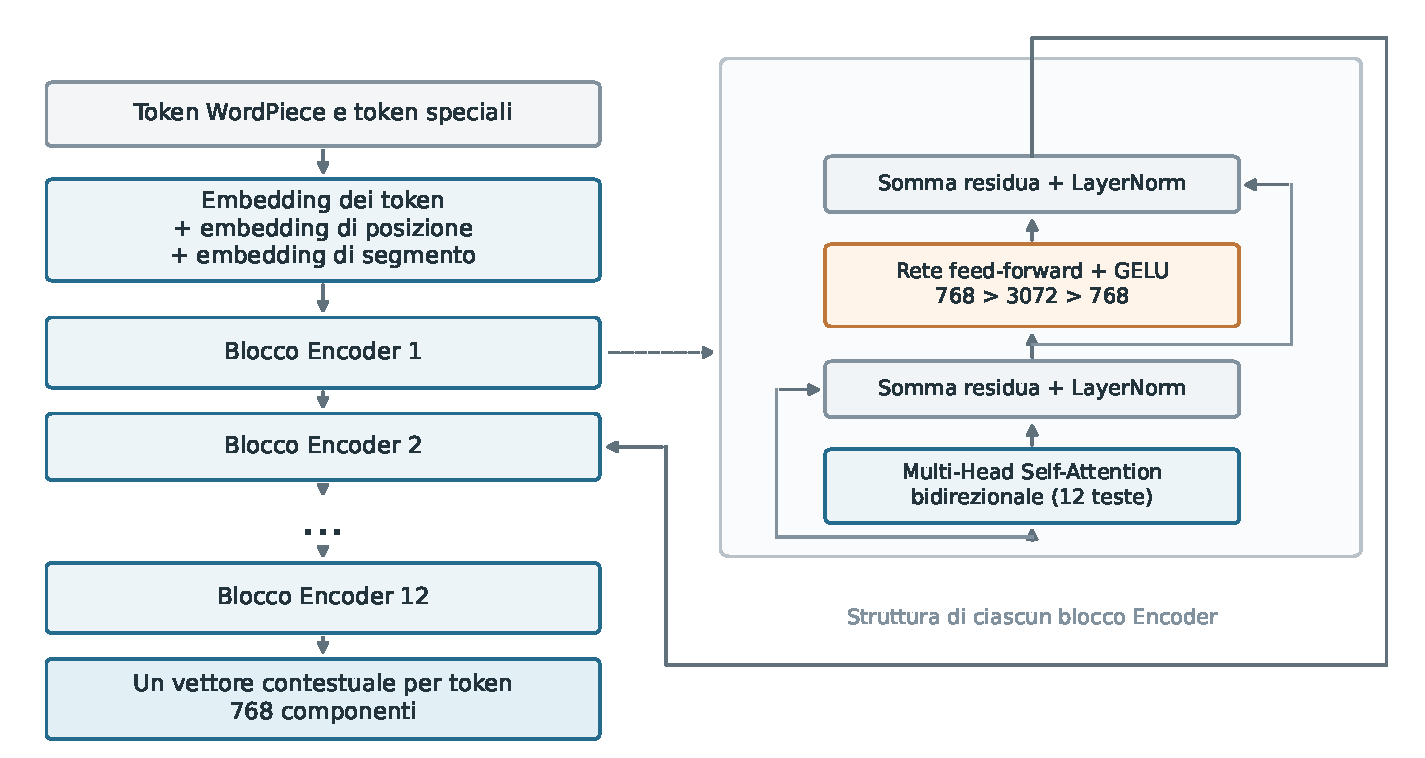
\includegraphics[width=0.90\textwidth]{figures/bert_encoder_structure.pdf}
\caption{Struttura dell'encoder BERT-Base utilizzato nel progetto, con 12 teste di attenzione per blocco e vettori di 768 componenti. A sinistra, il flusso delle rappresentazioni procede dall'alto verso il basso attraverso i 12 blocchi; a destra, la struttura interna comune a tutti i blocchi, con attenzione bidirezionale, rete feed-forward e connessioni residue. La freccia di uscita mostra, come esempio, il passaggio dal primo al secondo blocco. Schema basato sull'architettura descritta da Devlin et al.~\cite{devlin2019}.}
\label{fig:bert-encoder-structure}
\end{figure}

Ogni blocco comprende una Multi-Head Self-Attention e una rete feed-forward. La prima esegue più operazioni di attenzione in parallelo, mediante proiezioni query, key e value apprese per ciascuna testa. Le uscite vengono concatenate e proiettate nello spazio di dimensione 768~\cite{vaswani2017}. Per ciascuna testa, l'attenzione è calcolata come:

\begin{equation}
\label{eq:scaled-dot-product-attention}
    \operatorname{Attention}(Q,K,V) =
    \operatorname{softmax}\!\left(
    \frac{QK^{\mathsf T}}{\sqrt{d_k}}
    \right)V,
\end{equation}

dove $Q$, $K$ e $V$ sono matrici ottenute mediante proiezioni lineari apprese delle rappresentazioni in ingresso:
\begin{itemize}
    \item \textbf{Query ($Q$):} rappresentano le informazioni ricercate dai token;
    \item \textbf{Key ($K$):} rappresentano le caratteristiche utilizzate per calcolare la compatibilità con le query;
    \item \textbf{Value ($V$):} contengono le informazioni da aggregare mediante i pesi di attenzione.
\end{itemize}

Il prodotto $QK^{\mathsf T}$ determina i punteggi di compatibilità, scalati per $\sqrt{d_k}$, dove $d_k=768/12=64$ è la dimensionalità delle key per ciascuna testa. La softmax normalizza tali punteggi in pesi di attenzione, utilizzati per calcolare una combinazione pesata dei vettori value.

La rete feed-forward applica indipendentemente a ciascun token due trasformazioni lineari, da 768 a 3\,072 componenti e viceversa, separate da un'attivazione GELU. Entrambi i sottolivelli impiegano dropout, connessioni residue e Layer Normalization per favorire la regolarizzazione e la stabilità dell'addestramento~\cite{devlin2019,vaswani2017}. Al termine dei 12 blocchi, l'encoder restituisce un vettore contestuale di 768 componenti per ciascun token, utilizzabile nei compiti supervisionati.

\subsection{Preaddestramento}
\label{subsec:pretraining}

Nel BERT originale il preaddestramento combina il Masked Language Modeling (MLM) e la Next Sentence Prediction (NSP). Nel MLM viene selezionato casualmente il 15\% dei token della sequenza: di questi, l'80\% viene sostituito con il token speciale \texttt{[MASK]}, il 10\% con un token casuale e il restante 10\% rimane invariato. Il modello deve predire i token originali nelle posizioni selezionate, sfruttando il contesto bidirezionale. La NSP richiede invece di determinare se due segmenti di testo siano consecutivi nel corpus, mediante una classificazione binaria~\cite{devlin2019}.

Attraverso il preaddestramento, BERT apprende rappresentazioni linguistiche contestuali da grandi quantità di testo, che possono successivamente essere adattate a diversi compiti supervisionati mediante fine-tuning. In particolare, il checkpoint adottato è stato preaddestrato su corpora italiani e mantiene la distinzione tra lettere maiuscole e minuscole durante la tokenizzazione~\cite{bertxxl}.

\section{Architettura ELECTRA}
\label{sec:electra-architecture}

ELECTRA è un modello basato su un Transformer Encoder bidirezionale, che produce una rappresentazione contestuale per ciascun token. Come in BERT, ogni posizione può utilizzare le informazioni presenti sia prima sia dopo di essa nella frase. La differenza principale riguarda l'obiettivo di preaddestramento, basato sul riconoscimento dei token sostituiti~\cite{electra2020}.

\subsection{Tokenizzazione}
\label{subsec:electra-tokenization}

Il checkpoint \modelid{dbmdz/electra-base-italian-xxl-cased-discriminator} utilizza una tokenizzazione WordPiece, mantenendo le parole intere oppure suddividendole in subword. La variante \emph{cased} conserva la distinzione tra lettere maiuscole e minuscole~\cite{electramodel}. La segmentazione in subword richiede di ricondurre le rappresentazioni dei token alle parole annotate nel corpus, come avviene per BERT; il metodo adottato nel progetto è descritto nella Sezione~\ref{sec:pooling}.

\subsection{Struttura dell'encoder}
\label{subsec:electra-encoder-structure}

Il discriminatore italiano adotta una configurazione con 12 blocchi Transformer Encoder, 12 teste di attenzione per blocco e rappresentazioni di dimensione 768~\cite{electramodel}. Gli embedding dei token sono combinati con quelli posizionali e di segmento; ciascun blocco comprende self-attention bidirezionale, rete feed-forward, connessioni residue e normalizzazione, secondo la struttura illustrata per BERT nella Figura~\ref{fig:bert-encoder-structure}~\cite{electra2020}.

L'encoder restituisce un vettore contestuale per ciascuna subword. La testa utilizzata nel preaddestramento effettua una classificazione binaria per posizione; per il PoS tagging viene sostituita da una testa supervisionata che predice le categorie UPOS. L'encoder mantiene quindi la capacità di rappresentare il contesto, mentre cambia il compito richiesto al classificatore.

\subsection{Preaddestramento}
\label{subsec:electra-pretraining}

Il preaddestramento di ELECTRA, denominato \emph{replaced token detection}, impiega un generatore e un discriminatore. Il generatore apprende a ricostruire token mascherati e propone sostituzioni plausibili; il discriminatore riceve la sequenza così modificata e deve riconoscere, in ogni posizione, se il token coincide con quello originale oppure è stato sostituito. Se il generatore ricostruisce il token corretto, la posizione viene considerata originale~\cite{electra2020}.

L'obiettivo del discriminatore utilizza tutte le posizioni della sequenza, anziché soltanto quelle selezionate per il mascheramento. Al termine del preaddestramento il generatore viene scartato e il discriminatore viene adattato ai compiti supervisionati. Il checkpoint impiegato nel progetto è stato preaddestrato sul corpus italiano XXL~\cite{electra2020,electramodel}.

\section{Architettura Qwen}
\label{sec:qwen-architecture}

Qwen2.5 è una famiglia di modelli linguistici autoregressivi basati su Transformer Decoder. A differenza degli encoder bidirezionali, il decoder applica un vincolo causale: ogni posizione può utilizzare soltanto i token precedenti e quello corrente. Il modello costruisce così una sequenza predicendo un token alla volta~\cite{qwen2024}.

\subsection{Tokenizzazione}
\label{subsec:qwen-tokenization}

Qwen2.5 utilizza una variante byte-level di Byte-Pair Encoding (BPE), che rappresenta il testo mediante unità ottenute da fusioni di sequenze di byte frequenti. Una parola può corrispondere a uno o più token, senza che tali unità coincidano necessariamente con le parole del corpus~\cite{qwen2024}. Anche la risposta contenente i tag UPOS viene tokenizzata: una singola etichetta può essere suddivisa in più token del modello.

La variante Instruct rappresenta gli scambi mediante un formato di conversazione, distinguendo istruzioni di sistema, messaggio dell'utente e risposta del modello~\cite{qwenmodel}. Nel progetto l'istruzione richiede di annotare le parole numerate e di restituire soltanto una lista JSON di tag; la frase occupa il messaggio dell'utente. Il formato concreto dell'input e della risposta è descritto nella Sezione~\ref{subsec:qwen-checkpoint}.

\subsection{Struttura del decoder}
\label{subsec:qwen-decoder-structure}

Il checkpoint Qwen2.5-1.5B-Instruct contiene circa 1,54 miliardi di parametri e 28 blocchi Transformer Decoder, con rappresentazioni di dimensione 1\,536. L'attenzione utilizza 12 teste query e 2 teste key/value mediante \emph{Grouped Query Attention} (GQA): più teste query condividono le stesse proiezioni key e value~\cite{qwenmodel,qwen2024}.

Ogni blocco combina attenzione causale, rete feed-forward con attivazione SwiGLU, connessioni residue e normalizzazione RMSNorm. La posizione dei token viene rappresentata mediante codifiche rotatorie RoPE~\cite{qwen2024}. Il calcolo dell'attenzione segue il principio dell'Equazione~\ref{eq:scaled-dot-product-attention}, ma maschera le posizioni successive al token considerato, impedendo di utilizzare testo non ancora generato. La rappresentazione finale alimenta una proiezione sul vocabolario, dalla quale si ricava la distribuzione del token successivo.

Nel PoS tagging l'intera frase viene fornita prima della risposta. Ogni tag generato può quindi dipendere da tutte le parole in ingresso e dai tag già prodotti, pur mantenendo il vincolo causale del decoder.

\subsection{Preaddestramento e adattamento a istruzioni}
\label{subsec:qwen-pretraining}

Il preaddestramento di Qwen apprende a predire il token successivo su grandi quantità di testo multilingue. Le sequenze testuali forniscono direttamente i bersagli di apprendimento, consentendo al modello di acquisire regolarità linguistiche e conoscenze utilizzabili in compiti diversi~\cite{qwen2024}.

La variante Instruct riceve inoltre un adattamento successivo al preaddestramento volto a seguire istruzioni e produrre risposte coerenti con il formato richiesto~\cite{qwen2024,qwenmodel}. Nel presente progetto questo checkpoint viene ulteriormente specializzato mediante fine-tuning supervisionato sulle sequenze di tag UPOS. L'adattamento QLoRA e la loss applicata alla risposta sono descritti nella Sezione~\ref{sec:qwenloss}.


\section{Obiettivi del progetto}
L'obiettivo è confrontare tre checkpoint preaddestrati distinti sullo stesso compito e sullo stesso corpus: due encoder con classificazione per parola e un modello che genera le etichette. La domanda riguarda la correttezza e gli errori dei sistemi ottenuti con il protocollo adottato, insieme al costo dell'adattamento e dell'inferenza.

Un secondo obiettivo è studiare il contributo dell'informazione sulle maiuscole. L'ablation confronta, per ogni modello, una configurazione addestrata sul testo originale e una addestrata sul testo minuscolo. La stessa trasformazione si applica ai dati di selezione e di valutazione, conservando parole, ordine e categorie gold.

Il progetto riutilizza dal lavoro NLP la segmentazione gold e l'analisi per categoria. I nuovi checkpoint, il pooling e l'ablation richiedono nuovi training e valutazioni. Il piano esclude l'encoder congelato; l'eventuale CRF resta uno sviluppo opzionale.

\chapter{Task, dati e metriche}
\label{chap:data-metrics}
\section{Definizione del task}
Ogni esempio è una frase $x=(w_1,\ldots,w_n)$ con una sequenza di etichette gold $y=(y_1,\ldots,y_n)$, dove $y_i$ appartiene all'inventario UPOS $C$. Il sistema deve restituire esattamente un'etichetta per ciascuna parola e nello stesso ordine. Non si richiede di ricostruire le parole né di identificare confini di frase.

Questa impostazione assume una segmentazione gold. Le prestazioni descrivono l'etichettatura di parole già individuate e non un sistema completo a partire da testo grezzo. Nei file CoNLL-U si considerano le parole sintattiche con identificativo intero, distinguendole dalle righe relative a token multiparola e nodi vuoti~\cite{conllu}.

\section{Corpus e provenienza dei dati}
\label{sec:data-provenance}
Il corpus è UD Italian-ISDT, release 2.15~\cite{isdt}. Per il progetto AI la fonte di caricamento è la distribuzione Hugging Face \modelid{universal-dependencies/universal_dependencies}, configurazione \texttt{it\_isdt}~\cite{hfdata}. Si fissa il tag \path{ud2.15-loader-v2.3.0} alla revisione immutabile \path{8426077f2e778f20d46a5b89a187e4f991cfe6c4}, con dati Parquet e categorie UPOS rappresentate come stringhe. Il numero di versione del loader, 2.3.0, è distinto dalla release 2.15 delle annotazioni.

Si mantengono gli split ufficiali: training per l'aggiornamento dei parametri, development per la selezione e test per la valutazione finale. Al caricamento si controllano la corrispondenza tra parole ed etichette, l'ordine delle frasi e la provenienza. Un hash della rappresentazione canonica di ciascuno split permette di individuare modifiche ai dati; le due condizioni dell'ablation condividono la stessa sequenza di etichette gold.

La distribuzione Hugging Face è stata confrontata con i file CoNLL-U ISDT 2.15 del progetto NLP: frasi, parole, etichette UPOS e ordine coincidono in tutti e tre gli split. La Tabella~\ref{tab:data} ne riporta i conteggi verificati. La cella di preparazione dei dati nel notebook controlla l'allineamento e registra hash e conteggi nel manifest generato automaticamente. L'identità dei dati consente di mantenere il benchmark, ma non rende riutilizzabili come nuovi risultati le predizioni dei precedenti checkpoint.

\begin{table}[!htbp]
\centering
\begin{tabular}{lrrr}
\toprule
Split & Frasi & Parole & Tag UPOS presenti\\
\midrule
Training & 13\,121 & 276\,014 & 17\\
Development & 564 & 11\,907 & 17\\
Test & 482 & 10\,417 & 15\\
\bottomrule
\end{tabular}
\caption{Dimensioni verificate del corpus HF ISDT 2.15. Il test non contiene occorrenze gold di \texttt{INTJ} e \texttt{PART}.}
\label{tab:data}
\end{table}

Il caricamento richiede la revisione fissata. In assenza della risorsa attesa, l'esecuzione deve interrompersi, senza sostituire silenziosamente il corpus con una release diversa o con un'altra fonte. I conteggi e gli hash della preparazione vengono conservati nel manifest del nuovo progetto.

Gli inventari delle classi vengono costruiti dal training. Il development e il test non contribuiscono alla scelta delle categorie disponibili al classificatore. Il campo \texttt{FEATS}, i lemmi e le dipendenze non sono forniti ai modelli come input, poiché contengono annotazioni ulteriori rispetto alle parole da classificare.

\section{Metriche di valutazione}
\label{sec:metrics}
Le metriche vengono definite in questa sezione prima di impiegarle nella selezione dei checkpoint e nell'interpretazione del confronto. Tutte le misure grammaticali sono calcolate sulle parole gold, con gli stessi inventari e le stesse convenzioni per i tre sistemi~\cite{sklearnmetrics}.

\subsection{Accuracy}
L'accuracy misura la frazione di parole con etichetta predetta uguale a quella di riferimento. Indicando con $N$ il numero totale di parole e con $\hat y_i$ la predizione, si definisce
\begin{equation}
\operatorname{Acc}=\frac{1}{N}\sum_{i=1}^{N}\mathbf{1}[\hat y_i=y_i].
\end{equation}
Ogni parola pesa allo stesso modo. Le classi frequenti contribuiscono quindi più delle classi rare al valore complessivo.

\subsection{Precision, recall e macro-F1}
Per ogni categoria $k$, $TP_k$ conta le predizioni corrette della classe, $FP_k$ le parole predette come $k$ con gold diverso e $FN_k$ le parole con gold $k$ assegnate a un'altra classe. Precision e recall sono
\begin{equation}
 P_k=\frac{TP_k}{TP_k+FP_k},\qquad
 R_k=\frac{TP_k}{TP_k+FN_k}.
\end{equation}
La precision descrive l'affidabilità delle predizioni della classe; la recall descrive quante sue occorrenze vengono riconosciute. Il loro compromesso è espresso dall'F1:
\begin{equation}
 F_{1,k}=\frac{2TP_k}{2TP_k+FP_k+FN_k},\qquad
 F_1^{\mathrm{macro}}=\frac{1}{|C|}\sum_{k\in C}F_{1,k}.
\end{equation}
Ogni rapporto con denominatore nullo viene posto a zero. La macro-F1 assegna lo stesso peso a ciascuna categoria, rendendo visibili difficoltà che l'accuracy può attenuare quando riguardano classi rare.

Si riportano due inventari per la media. La \emph{macro-F1 totale} utilizza tutti i diciassette tag UPOS; la \emph{macro-F1 sulle classi presenti} considera i tag con supporto gold positivo nello split valutato. Entrambe mantengono nei conteggi gli errori verso categorie diverse. Le classi assenti hanno F1 nullo nella media totale, anche se non vengono mai predette: con $m$ classi gold presenti su diciassette il massimo della media totale è pertanto $m/17$. Nel test verificato sono presenti quindici classi, per cui il massimo della macro-F1 totale è $15/17\simeq88{,}24\%$, mentre la media sulle classi presenti può raggiungere il 100\%.

La macro-F1 totale sul development è la misura adottata per selezionare i checkpoint. L'accuracy, la macro-F1 sulle classi presenti e le misure per categoria completano la valutazione finale. Le loss dei modelli non sostituiscono queste metriche comuni.

\subsection{Validità delle risposte generative}
Una risposta Qwen è valida se contiene soltanto una lista JSON di stringhe con un tag UPOS riconosciuto per ogni parola gold, nell'ordine richiesto. Testo aggiuntivo, numero errato di elementi o etichette non ammesse rendono invalida l'intera risposta.

In tal caso si assegna \invalid\ a tutte le parole della frase: ciascuna conta come errore nell'accuracy e falso negativo della propria categoria nell'F1. La frase rimane nella valutazione. Il \emph{tasso di risposte invalide} è la frazione di frasi con output non valido. Queste regole si applicano anche alla selezione sul development.

Una lista valida può comunque contenere tag errati: il tasso di invalidità affianca le metriche UPOS, che comprendono tutte le frasi.

\subsection{Aggregazione e variazioni appaiate}
Per ciascun modello e condizione si riportano media e deviazione standard campionaria sui seed 42, 123 e 456, conservando anche le singole misure~\cite{seeds}. L'effetto dell'ablation viene espresso in punti percentuali mediante
\begin{equation}
\Delta_{s}=100\bigl(M_{\mathrm{minuscolo},s}-M_{\mathrm{originale},s}\bigr),
\end{equation}
dove $M$ è una metrica in $[0,1]$. Un valore negativo segnala una riduzione dopo la rimozione delle maiuscole. Le differenze appaiate vengono riassunte con media e deviazione standard; tre seed descrivono solo parte della variabilità del training.

\chapter{Modelli e funzioni obiettivo}
\label{chap:models}
\section{Scelta dei checkpoint}
Il confronto usa tre checkpoint distinti, riassunti nella Tabella~\ref{tab:models}. La selezione privilegia modelli adattabili su una singola GPU e differenze che abbiano un significato per il task: due encoder italiani con diversa procedura di preaddestramento e un sistema generativo multilingue.

\begin{table}[!htbp]
\centering\small
\begin{tabularx}{\textwidth}{>{\raggedright\arraybackslash}p{2.5cm}>{\raggedright\arraybackslash}X>{\raggedright\arraybackslash}X}
\toprule
Modello & Checkpoint Hugging Face & Adattamento\\
\midrule
BERT XXL italiano & \modelid{dbmdz/bert-base-italian-xxl-cased} & Fine-tuning dell'encoder e della testa UPOS\\[3pt]
ELECTRA XXL italiano & \modelid{dbmdz/electra-base-italian-xxl-cased-discriminator} & Fine-tuning dell'encoder e della testa UPOS\\[3pt]
Qwen2.5-1.5B-Instruct & \modelid{Qwen/Qwen2.5-1.5B-Instruct} & Fine-tuning supervisionato con adapter LoRA e pesi di base quantizzati\\
\bottomrule
\end{tabularx}
\caption{Modelli del confronto principale. Le revisioni immutabili dei checkpoint sono fissate nella configurazione del notebook e conservate negli output di esecuzione.}
\label{tab:models}
\end{table}

\subsection{BERT XXL italiano}
Il checkpoint BERT XXL adotta la configurazione BERT-Base descritta nella Sezione~\ref{sec:bert-architecture}. La sigla XXL identifica la variante preaddestrata su un corpus italiano ampliato con OSCAR, per circa 81 GB di testo secondo gli autori; non indica un encoder con molti più strati~\cite{bertxxl}. Il modello mantiene la distinzione tra maiuscole e minuscole e permette di studiare l'effetto della loro rimozione.

\subsection{ELECTRA XXL italiano}
Si utilizza il checkpoint italiano del discriminatore descritto nella Sezione~\ref{sec:electra-architecture}, sostituendo la testa di preaddestramento con il classificatore UPOS~\cite{electramodel}.

Il corpus italiano XXL e la forma dell'output per parola rendono ELECTRA un confronto pertinente per BERT. Tuttavia, checkpoint, ottimizzazione di preaddestramento e rappresentazioni non coincidono: gli scarti finali non isolano causalmente il solo obiettivo di preaddestramento. Nel fine-tuning si mantiene la stessa strategia di pooling e la stessa forma della testa per ridurre differenze introdotte dal codice del task.

\subsection{Qwen2.5-1.5B-Instruct}
\label{subsec:qwen-checkpoint}
Per il modello generativo si adotta la variante Instruct descritta nella Sezione~\ref{sec:qwen-architecture}. La model card dichiara supporto multilingue, compreso l'italiano, e adattamento a istruzioni e output strutturati~\cite{qwenmodel}. Queste caratteristiche motivano l'impiego di una risposta JSON, ma non garantiscono la correttezza del tagging: formato e categorie vengono verificati separatamente.

L'input elenca le parole gold con un indice progressivo e richiede solo la lista dei tag, evitando di far rigenerare le parole. Ad esempio, per «Il gatto dorme» si forniscono \texttt{1: Il}, \texttt{2: gatto}, \texttt{3: dorme} e si richiede la risposta \texttt{["DET", "NOUN", "VERB"]}. Questo esempio illustra il formato; il training utilizza le annotazioni reali del corpus.

\section{Allineamento e mean pooling}
\label{sec:pooling}
I tokenizer degli encoder suddividono alcune parole in più subword. Il task possiede però una sola etichetta per parola. Il tokenizer fast restituisce mediante \texttt{word\_ids} l'associazione tra ogni subword e la parola di origine~\cite{hfclassification}. Tale associazione viene conservata per tutte le subword e verificata prima del training.

Indicando con $S_i$ l'insieme delle posizioni associate alla parola $w_i$ e con $h_j\in\mathbb{R}^{d}$ il vettore finale dell'encoder alla posizione $j$, la rappresentazione della parola è
\begin{equation}
\label{eq:meanpool}
z_i=\frac{1}{|S_i|}\sum_{j\in S_i}h_j.
\end{equation}
Il pooling precede dropout e testa lineare. Token speciali e padding non appartengono ad alcun $S_i$ e non contribuiscono alla media. Il classificatore riceve una sequenza di parole, mentre il modello di linguaggio elabora la sequenza di subword.

La media aggrega esplicitamente tutti i frammenti della parola e mantiene invariata la dimensione del vettore, senza introdurre parametri aggiuntivi. Ogni parola contribuisce una sola volta alla loss e alle metriche, indipendentemente dal numero di frammenti. Questa scelta offre una base semplice e condivisa per i due encoder.

La supervisione sulla sola prima subword è una strategia alternativa diffusa~\cite{hfclassification}. Non equivale a eliminare dal modello i frammenti successivi: la prima rappresentazione è già contestualizzata dalla self-attention. Il mean pooling viene adottato per rendere esplicita l'aggregazione e non perché il metodo precedente ricevesse soltanto il prefisso della parola. La letteratura mostra che l'aggregazione può influire sulle prestazioni in modo dipendente da task e modello~\cite{acs2021}; non dimostra che la media sia necessariamente ottimale nel presente esperimento.

La lunghezza massima degli encoder è fissata a 512 subword, inclusi i token speciali. L'audit dei tokenizer copre tutte le frasi: la sequenza più lunga richiede 332 posizioni nella condizione originale e 331 in minuscolo. Il preprocessing verifica la copertura di ogni parola e interrompe l'esecuzione in caso di superamento del limite, evitando troncature silenziose.

Per Qwen si considera l'intera sequenza di prompt e risposta gold. Sul training la lunghezza massima è 2\,907 token con testo originale e 2\,897 in minuscolo. Si adotta quindi un limite di 3\,072 token, sufficiente anche per development e test. La scelta deriva dalla copertura del training; il controllo sugli altri split verifica l'assenza di troncature, senza usare la correttezza delle predizioni per ottimizzare il modello. La sezione di allineamento del notebook contiene i controlli di copertura dei tokenizer.

\section{Loss degli encoder}
\label{sec:encoderloss}
La testa lineare trasforma $z_i$ in uno score per ognuna delle diciassette categorie. La softmax produce la distribuzione $p_\theta(k\mid x,i)$. L'obiettivo supervisionato è la cross-entropy:
\begin{equation}
\label{eq:encoderloss}
\mathcal{L}_{\mathrm{UPOS}}=-\frac{1}{N_B}\sum_{i\in B}\log p_\theta(y_i\mid x,i),
\end{equation}
dove $B$ comprende le parole valide del batch su cui viene calcolata la loss e $N_B$ è il loro numero. Il padding è escluso mediante maschera o etichetta di ignoramento~\cite{torchce}. L'aggiornamento dei parametri e l'eventuale accumulo dei gradienti sono gestiti dal \texttt{Trainer}.

Questa loss coincide con la log-verosimiglianza negativa delle categorie gold sotto la fattorizzazione adottata dal classificatore. È una scelta naturale per un problema multiclasse con una sola etichetta corretta per parola e consente di aggiornare sia la testa sia l'encoder. La predizione seleziona la categoria con score massimo.

Il piano iniziale non applica pesi di classe o label smoothing. Questa impostazione mantiene un obiettivo semplice e uguale per i due encoder; le difficoltà sulle categorie rare vengono osservate tramite la macro-F1 e l'analisi per classe. Eventuali pesi dovrebbero essere ricavati dal training e valutati sul development, costituendo una modifica ulteriore da documentare.

Non si eredita la combinazione di loss UPOS e FEATS del precedente progetto. Con il solo UPOS non esistono coefficienti per bilanciare compiti diversi: il peso manuale della loss morfologica non appartiene quindi al nuovo esperimento principale.

\section{Loss generativa e adattamento QLoRA}
\label{sec:qwenloss}
Nel fine-tuning di Qwen la frase e l'istruzione costituiscono il prompt $x$; la risposta gold $a=(a_1,\ldots,a_T)$ contiene la lista JSON dei tag. Il training usa teacher forcing, fornendo i token gold precedenti per predire il successivo:
\begin{equation}
\label{eq:qwenloss}
\mathcal{L}_{\mathrm{gen}}=-\frac{1}{T_B}\sum_{t\in A_B}\log p_\theta(a_t\mid x,a_{<t}),
\end{equation}
dove $A_B$ contiene le posizioni valide della risposta e $T_B=|A_B|$. I token del prompt e del padding hanno etichetta \texttt{-100} e non contribuiscono alla loss~\cite{trlsft}. La risposta include anche punteggiatura JSON e terminazione: l'obiettivo apprende sia le categorie sia il formato richiesto. Si utilizza la loss causale fornita dal modello Hugging Face; l'accumulo dei gradienti segue la gestione del \texttt{Trainer}, con otto microbatch per aggiornamento nella configurazione iniziale.

La media è qui calcolata sui token testuali della risposta, non sulle parole del corpus. Un tag può essere rappresentato da più token del tokenizer Qwen. Per questa ragione, e per la diversa fattorizzazione probabilistica, i valori numerici di $\mathcal{L}_{\mathrm{gen}}$ e $\mathcal{L}_{\mathrm{UPOS}}$ non vanno confrontati come misure della qualità dei sistemi. Il confronto finale usa le metriche UPOS della Sezione~\ref{sec:metrics}.

LoRA rappresenta l'aggiornamento di una matrice preaddestrata $W_0$ mediante un prodotto a rango ridotto, $W=W_0+(\alpha/r)BA$, mantenendo fissi i pesi di base e addestrando gli adapter~\cite{lora2022}. QLoRA combina tale adattamento con la quantizzazione dei pesi di base a 4 bit~\cite{qlora2023,peftquant}. Il rango iniziale è $r=16$, con $\alpha=32$ e dropout degli adapter pari a 0,05. Gli adapter interessano le trasformazioni lineari compatibili dell'architettura; la configurazione usa quantizzazione NF4 con doppia quantizzazione e gradient checkpointing per ridurre la memoria delle attivazioni.

La scelta riduce il numero di parametri aggiornati e il consumo di memoria rispetto al fine-tuning completo del generativo. Il riferimento hardware è una RTX 4070 SUPER con 12 GB di memoria: la dimensione del batch e la lunghezza massima devono comunque essere controllate mediante una prova breve, poiché attivazioni, precisione e optimizer contribuiscono al consumo effettivo. La fattibilità non viene dedotta dal solo numero di parametri.

QLoRA è fine-tuning con parametri addestrabili negli adapter. La differenza rispetto all'aggiornamento completo degli encoder fa parte delle condizioni del confronto e deve accompagnarne le conclusioni. Non si interpreta uno scarto tra Qwen e BERT come effetto isolato dell'architettura o della sola dimensione del modello.

\chapter{Protocollo sperimentale}
\label{chap:protocol}
\section{Configurazioni e impostazioni iniziali}
Il piano comprende tre modelli, due condizioni di input e tre seed, per un totale di $3\times2\times3=18$ training. Ogni esecuzione parte dal checkpoint preaddestrato corrispondente e salva configurazione, revisione delle risorse, versioni delle librerie e hash dei dati. Le directory, raccolte in \path{outputs/upos_trainer_v1/}, distinguono modello, condizione e seed.

Il notebook \path{notebooks/Italian_UPOS_AI.ipynb} estende \path{BERT_Italian_PoS_UD_2_15.ipynb} del progetto NLP, conservandone struttura e logica di esecuzione. Le sezioni seguono lo stesso ordine: ambiente, configurazione, dati, tokenizzazione, metriche, modelli, training, valutazione, confronto e analisi degli errori. L'esecuzione della cella di training avvia direttamente i sistemi e i seed configurati e riutilizza i training già completati. Il ciclo di ottimizzazione utilizza Hugging Face \texttt{Trainer}, con barre di avanzamento, valutazione periodica e salvataggio dei checkpoint.

\begin{table}[!htbp]
\centering\small
\begin{tabularx}{\textwidth}{Xcc}
\toprule
Impostazione & BERT ed ELECTRA & Qwen\\
\midrule
Epoche massime & 10 & 3\\
Learning rate & $2\cdot10^{-5}$ & $2\cdot10^{-4}$\\
Batch di training per dispositivo & 8 & 1\\
Accumulo dei gradienti & 1 & 8\\
Batch di valutazione & 16 & 1\\
Limite della sequenza & 512 subword & 3\,072 token\\
Adattamento & Parametri completi & Adapter QLoRA\\
Rango / scala LoRA & -- & $16$ / $32$\\
Dropout LoRA & -- & $0{,}05$\\
Seed & \multicolumn{2}{c}{42, 123, 456}\\
\bottomrule
\end{tabularx}
\caption{Configurazione iniziale. I limiti di sequenza derivano dall'audit di copertura del corpus; gli iperparametri di ottimizzazione costituiscono un punto di partenza e non valori ottimali individuati sperimentalmente.}
\label{tab:training}
\end{table}

L'ottimizzazione utilizza AdamW, che separa la penalizzazione dei pesi dall'aggiornamento adattivo~\cite{adamw2019}. Per gli encoder si impiegano weight decay 0,01, warmup pari al 10\% dei passi e dropout 0,1. La cella di configurazione del notebook definisce le impostazioni complete; ogni esecuzione le conserva insieme alla provenienza dei dati e agli argomenti del \texttt{Trainer}. Precisione numerica e scheduler vengono registrati con le informazioni di training. Il seed viene impostato prima dell'inizializzazione della nuova testa o degli adapter e controlla le principali operazioni stocastiche, compreso l'ordine dei batch.

I budget sono mantenuti uguali tra testo originale e minuscolo per lo stesso modello. Tra encoder e generativo si usano impostazioni differenti, motivate dalla diversa dimensione e dal tipo di adattamento. Il confronto riguarda quindi sistemi addestrati con risorse dichiarate; non è un esperimento a identico numero di parametri aggiornati, identico numero di token o identico costo computazionale.

Le impostazioni potranno essere riviste sul development prima della campagna definitiva. Una modifica comporta una nuova configurazione identificabile e non sovrascrive i risultati già prodotti. Il test non guida learning rate, numero di epoche, formato del prompt o scelta della regola per gli output invalidi.

\section{Selezione del checkpoint e inferenza}
\label{sec:selection}
Al termine di ogni epoca il \texttt{Trainer} valuta il modello sul development e salva un checkpoint. Per tutti i modelli si seleziona quello con la macro-F1 totale UPOS più alta, definita nella Sezione~\ref{sec:metrics}, e lo si ricarica al termine del training. Questo criterio privilegia una lettura per categoria e mantiene la stessa misura di selezione tra classificatori e sistema generativo.

Per gli encoder si calcolano i tag a partire dagli score per parola. Per Qwen il punteggio development richiede una vera generazione autoregressiva: il modello produce la risposta senza ricevere i tag gold precedenti. La loss in teacher forcing è utile per seguire l'ottimizzazione ma non rappresenta la qualità della generazione libera e non viene usata come sostituto della metrica comune.

La generazione deve avere una configurazione riproducibile, registrando strategia di decodifica, limite dei token nuovi e token di terminazione. Il protocollo iniziale usa decodifica deterministica. Il limite di generazione non deve troncare le liste più lunghe del corpus: la preparazione verifica le lunghezze gold e l'esecuzione conserva eventuali terminazioni incomplete come output invalidi.

Dopo il completamento dei training, la sezione di valutazione ricarica i modelli selezionati e applica il metodo \texttt{predict} del \texttt{Trainer} al test, una volta per ciascun run. Per Qwen il passo di predizione esegue la generazione autoregressiva. Il test non viene usato per scegliere tra epoche dello stesso training. Metriche e predizioni vengono conservate nei file del run, così le sezioni successive possono ricalcolare confronto e analisi degli errori senza ripetere l'inferenza.

\section{Ablation dell'informazione sulle maiuscole}
\label{sec:ablation}
L'ablation interviene su una feature dell'input condivisa dai tre modelli. Nella condizione \emph{originale} si conservano le forme del corpus; nella condizione \emph{minuscolo} si applica la conversione in minuscolo a ogni parola prima della tokenizzazione. La trasformazione riguarda training, development e test, mentre etichette, ordine delle parole e appartenenza agli split restano invariati.

\begin{table}[!htbp]
\centering
\begin{tabularx}{\textwidth}{Xcc}
\toprule
Modello & Testo originale & Testo minuscolo\\
\midrule
BERT XXL italiano & 3 seed & 3 seed\\
ELECTRA XXL italiano & 3 seed & 3 seed\\
Qwen2.5-1.5B-Instruct & 3 seed & 3 seed\\
\bottomrule
\end{tabularx}
\caption{Disegno dell'ablation comune: sei configurazioni e diciotto esecuzioni. Il confronto è appaiato per modello e seed.}
\label{tab:ablation}
\end{table}

L'ipotesi è che le maiuscole forniscano indizi utili per distinguere alcune categorie, soprattutto nomi propri e nomi comuni. Il segno e l'entità dell'effetto devono essere misurati: una configurazione potrebbe compensare la perdita di indizi usando il contesto o generalizzare diversamente dopo il riaddestramento.

La conversione può cambiare anche la suddivisione in subword e la frequenza di token poco rappresentati nel preaddestramento. L'esperimento misura pertanto l'effetto complessivo della rimozione delle maiuscole nel sistema, includendo il tokenizer. Non isola una rappresentazione astratta della capitalizzazione a parità di tokenizzazione.

Si confrontano modelli riaddestrati nelle due condizioni. Convertire soltanto il test di un modello addestrato sul testo originale risponderebbe invece a una domanda di robustezza rispetto a un cambiamento dell'input. Le due impostazioni non devono essere confuse nella descrizione dei risultati.

\section{Analisi degli errori e del costo}
Le confusioni vengono conteggiate sulle parole gold e aggregate per categoria predetta e corretta. Si esaminano in particolare gli scambi \texttt{NOUN}/\texttt{PROPN}, \texttt{AUX}/\texttt{VERB} e \texttt{ADJ}/\texttt{VERB}, conservando il contesto della frase e il supporto delle classi. Queste coppie sono categorie di analisi da verificare, non errori già osservati nei nuovi modelli.

L'analisi affianca casi condivisi da tutti i sistemi e casi in cui le predizioni differiscono. Gli esempi qualitativi devono essere selezionati con criteri dichiarati e accompagnati dall'annotazione gold; una parola ambigua o una convenzione del treebank può rendere fuorviante una spiegazione basata soltanto sulla forma isolata.

Per Qwen si distinguono risposte formalmente valide ma grammaticalmente errate e risposte invalide. In quest'ultimo gruppo si registrano separatamente fallimenti di parsing, numero errato di tag ed etichette sconosciute, pur applicando la stessa penalizzazione alle metriche comuni.

Il costo del sistema comprende tempo di training, numero di parametri aggiornati, memoria GPU osservata e tempo di inferenza sul medesimo test. Le misure devono indicare hardware, batch, precisione e inclusione di valutazioni e salvataggi. La generazione sequenziale dei tag e la classificazione parallela delle parole richiedono procedure diverse; i tempi appartengono all'analisi pratica del sistema e non sostituiscono le metriche linguistiche.

\chapter{Risultati e limiti del confronto}
\label{chap:results}
\section{Stato degli esperimenti}
Questa relazione documenta il protocollo e le scelte iniziali del nuovo progetto. Alla data del 24 novembre 2026 non sono disponibili risultati dei diciotto training completi previsti. Accuracy, macro-F1, differenze dell'ablation e costi effettivi devono essere ottenuti eseguendo il piano sulle risorse dichiarate.

I controlli di preparazione verificano allineamento e copertura delle parole prima del training; non misurano la qualità linguistica dei checkpoint fine-tunati. I risultati del progetto NLP precedente riguardano un diverso modello di partenza e una diversa aggregazione e non popolano le tabelle del nuovo confronto.

\section{Presentazione dei risultati finali}
La raccolta finale deve contenere una riga per modello, condizione e seed, con accuracy, macro-F1 totale, macro-F1 sulle classi presenti e, per Qwen, tasso di risposte invalide. Un riepilogo presenta medie e deviazioni standard, conservando le misure individuali per verificare se gli scarti siano uniformi tra seed.

L'ablation richiede una tabella di differenze appaiate e un'analisi delle categorie maggiormente interessate. Un calo della sola macro-F1 può dipendere da poche occorrenze di una classe rara; per interpretarlo si riportano supporti e conteggi di errore. Un vantaggio medio contenuto non prova una superiorità generale se varia tra esecuzioni o dipende da pochi esempi.

Le curve di training e development potranno mostrare evoluzione della loss e della macro-F1, con il checkpoint selezionato indicato esplicitamente. Per Qwen si deve distinguere la loss calcolata con teacher forcing dalla metrica ottenuta generando le liste. La lettura congiunta consente di individuare casi in cui l'ottimizzazione della probabilità dei token non corrisponde a un miglioramento del tagging libero.

\section{Limiti metodologici}
Il confronto usa un solo treebank italiano e segmentazione gold. Le conclusioni riguarderanno quindi quel dominio e quelle convenzioni, senza estendersi automaticamente a testi informali, altri corpora o input da segmentare. La possibile sovrapposizione tra dati pubblici e corpora di preaddestramento non è esclusa dal solo uso di split supervisionati separati.

I modelli differiscono per numero di parametri, tokenizer, preaddestramento e procedura di adattamento. BERT ed ELECTRA aggiornano l'encoder completo, mentre Qwen aggiorna adapter su pesi quantizzati. Il confronto è informativo sul risultato dei sistemi, ma non permette di attribuire uno scarto a una singola differenza architetturale.

Il criterio di invalidità applicato all'intera frase è conservativo: evita riallineamenti opportunistici degli output generativi e penalizza la mancata osservanza del formato. Al tempo stesso rende una risposta quasi corretta ma formalmente incompleta diversa da una lista valida con un solo tag errato. Il tasso di invalidità e l'ispezione degli output rendono esplicita questa componente del risultato.

Infine, tre seed non esauriscono tutte le fonti di incertezza. Il confronto appaiato rende visibile la variabilità tra esecuzioni; eventuali intervalli basati su ricampionamento delle frasi descriverebbero invece l'incertezza del test per predizioni già ottenute. Le due forme di variabilità devono rimanere distinte.

\chapter{Conclusioni e sviluppi}
Il progetto definisce un confronto riproducibile tra BERT XXL italiano, ELECTRA XXL italiano e Qwen2.5-1.5B-Instruct nel PoS tagging. I primi due modelli condividono una rappresentazione per parola costruita con mean pooling e una testa supervisionata; il generativo viene adattato a produrre direttamente la sequenza dei tag. Le rispettive loss sono motivate dal tipo di output e il confronto usa metriche grammaticali comuni.

L'ablation delle maiuscole introduce la stessa modifica dell'input per tutti i modelli e prevede il riaddestramento nelle due condizioni. Questa impostazione consente di studiare il contributo dell'informazione ortografica mantenendo invariati corpus, etichette e protocollo di ciascun modello. L'eventuale vantaggio di un sistema e l'entità dell'effetto dell'ablation restano risultati da misurare.

Un successivo approfondimento potrà valutare una CRF sugli encoder, confrontando classificazione indipendente e decodifica strutturata senza cambiare il pooling. Si tratterebbe di un'ablation architetturale aggiuntiva, distinta dallo studio comune sui dati e non inclusa nelle diciotto esecuzioni. Altri sviluppi possibili sono la supervisione morfologica, il confronto tra strategie di pooling e la valutazione su un diverso treebank, ciascuno con controlli dedicati.

\clearpage
\phantomsection
\addcontentsline{toc}{chapter}{\bibname}
\bibliographystyle{unsrturl}
{\footnotesize\raggedright\setlength{\parskip}{0pt}\interlinepenalty=10000\bibliography{references}}
\end{document}
